\documentclass[11pt]{article}

\usepackage[margin=1in]{geometry}
\usepackage{graphicx}
\usepackage{booktabs}
\usepackage{amsmath}
\usepackage{amssymb}
\usepackage{authblk}
\usepackage{orcidlink}
\usepackage[round,authoryear]{natbib}
\usepackage{hyperref}

\title{Noise-Dependent Advantages of Expectile over Quantile Learning in a Minimal Distributional Reinforcement Learning Model}

\author[1]{Z. Jana\orcidlink{0009-0009-3316-7476}}
\affil[1]{Department of Computer Science and Engineering,
The American University in Cairo}

\date{}

\begin{document}

\maketitle

\section{Introduction}
\label{sec:intro}

Classical accounts of reward-based learning in the brain treat the dopaminergic reward-prediction-error (RPE) signal as a teaching signal for a single scalar quantity: the mean of future expected reward. Distributional reinforcement learning (RL) departs from this picture by instead learning an entire probability distribution over returns, represented as a population of value predictors that differ in their degree of optimism \citep{bellemare2017}. \citet{dabney2020} provided the first strong evidence that this is not merely a machine-learning abstraction: dopamine neurons in mouse ventral tegmental area show exactly the diversity in reversal points predicted by a \emph{quantile}-based distributional code, in which each channel learns a different quantile of the reward distribution via an asymmetric (pinball-loss) update.

\citet{lowet2025} extended this line of evidence from midbrain dopamine to the striatum itself, and in doing so proposed a different algorithmic substrate. Recording striatal population activity while mice experienced cues predicting reward distributions that shared a mean but differed in variance, they found that variance is encoded abstractly (i.e., in an odor-identity-independent format) and that this coding is best explained not by quantile regression but by \emph{expectile} regression: an asymmetric \emph{squared}-loss analogue of quantile regression, in which each channel's prediction error is scaled by its magnitude rather than reduced to its sign \citep{rowland2019}. Crucially, they link this algorithmic choice to a specific piece of striatal anatomy: implementing expectile-based distributional RL with opponent, sign-flipped plasticity in D1- and D2-type medium spiny neurons (MSNs) --- reflected expectile distributional RL, or REDRL --- reproduces both the geometry of the population code and a battery of causal manipulations (dopamine lesion, optogenetics), and explains why D1 MSNs are systematically more optimistic and D2 MSNs more pessimistic than their dopaminergic inputs alone would predict.

This raises a question that neither the original expectile-regression theory nor its striatal instantiation directly addresses: \emph{why expectile, rather than quantile, regression?} \citet{rowland2019} show that expectiles are theoretically privileged in one specific sense --- a set of statistics is exactly learnable through recursive Bellman-style updates (``Bellman closed'') only if it is a set of moments, and the mean is recovered exactly by the $\tau=0.5$ expectile but not by any single quantile. Yet this is a statement about asymptotic, noise-free convergence; empirically, quantile-based distributional RL performs comparably well at scale, underlies the original dopamine evidence in \citet{dabney2020}, and quantile and expectile agents converge to correct answers under the same idealized conditions. If both algorithms are valid targets at convergence, Bellman closedness alone does not explain why a biological circuit constrained by noisy, non-stationary, finite experience would be better served by one over the other.

A parallel and largely independent literature has asked why the striatum's D1/D2 opponent architecture itself --- rather than expectile coding specifically --- would be favored by learning and choice. \citet{jaskirfrank2023} show that dynamic, environment-dependent modulation of D1 (``Go'') and D2 (``No-Go'') pathways solves an exploration problem: in reward-sparse environments, stochastic sampling noise can make the estimated value of the objectively best option fall below that of worse options, and opponent, environment-adaptive gain on the two pathways corrects for this. This is a compelling normative account of D1/D2 opponency, but it is not an account of why the \emph{loss function} governing each pathway's plasticity should be expectile-like in the first place --- nor does it address noise in the \emph{learning} signal itself, as opposed to noise in the environment's reward statistics. Separately, behavioral work on asymmetric learning rates ($\alpha^+ \ne \alpha^-$) shows that human participants exhibit systematic optimism or pessimism in exactly the way an expectile-like update predicts, and that this asymmetry is itself a stable, measurable individual trait \citep{lefebvre2017}, while other work shows that a substantial fraction of apparently ``exploratory'' human choice variability is in fact driven by computational noise intrinsic to the learning process, with measurable physiological correlates \citep{findling2019}. Taken together, these findings motivate treating learning-signal noise --- not just environmental stochasticity --- as a first-class constraint that any biologically plausible learning rule must tolerate.

Here we ask whether there is a normative, noise-dependent reason to prefer expectile over quantile updates, independent of their shared asymptotic validity. We build a minimal population of Rescorla--Wagner-style units with heterogeneous, asymmetric learning rates --- calibrated, but not fit, to the striatal recordings of \citet{lowet2025} --- and compare expectile and quantile update rules directly as we vary the amount of noise injected into the learning signal. We then ask whether the same property that governs any noise-dependent advantage also governs the emergence of D1/D2-like opponent geometry in the population, and whether an advantage observed in the model's internal representational geometry translates into better active decision-making across three qualitatively different task structures: tracking abrupt distributional shifts, tracking continuous drift, and identifying a high-value but high-variance option under resource pressure. Results are reported in Section~\ref{sec:results}; full model, task, and statistical details are given in Section~\ref{sec:methods}.

\section{Results}
\label{sec:results}

\subsection{A minimal population of asymmetric learners reproduces the qualitative signatures of striatal distributional coding}
\label{sec:results-baseline}

Before asking whether expectile and quantile learning rules differ in their robustness to noise, we first verified that a population of independent Rescorla--Wagner (RW) units with heterogeneous asymmetric learning rates reproduces, under clean (noise-free) conditions, the three qualitative signatures that motivate treating it as a plausible minimal model of the striatal population code: (i) an abstraction hierarchy across reward statistics, (ii) opponent geometry between optimistic and pessimistic subpopulations, and (iii) a behavioral readout that discriminates rewarded from unrewarded cues while remaining blind to reward variance.

Under the expectile update rule, the cross-condition-generalization abstraction index (AI; see Section~\ref{sec:methods-decoding}) followed the same rank order as the reference values obtained from real striatal recordings (Section~\ref{sec:methods-empirical}): mean AI $= 0.501 \pm 0.023$, variance AI $= 0.030 \pm 0.030$, kurtosis AI $= -0.009 \pm 0.027$ (mean $\pm$ SEM across $n=30$ seeds), against empirical reference values of $0.623$, $0.098$, and $0.006$, respectively. The corresponding parallelism (cosine-alignment) scores showed the same ordering (mean $0.714$, variance $0.024$, kurtosis $0.016$).

Splitting the population post hoc by the sign of each unit's effective expectile level ($\tau > 0.5$, ``D1-like'', optimistic, versus $\tau \le 0.5$, ``D2-like'', pessimistic) revealed clear opponent geometry with no D1/D2 architecture imposed: D1-like units placed the Variable cue reliably farther from Nothing than the Fixed cue ($d(N,\mathrm{Var}) - d(N,\mathrm{Fix}) = +2.111$, $p = 1.35\times10^{-18}$), while D2-like units showed the opposite pattern ($-2.525$, $p = 1.59\times10^{-17}$; one-sample $t$-tests against zero, $n=30$ seeds).

A linear delta-rule readout trained on the converged population activity discriminated rewarded (Fixed, Variable) from unrewarded (Nothing) cues (Nothing vs.\ Fixed: $\Delta = -3.803$, $p = 9.34\times10^{-6}$) but showed no reliable discrimination between Fixed and Variable cues (Fixed vs.\ Variable: $\Delta = -0.209$, $p = 0.281$), consistent with the behavioral blindness to reward variance reported for real animals performing the analogous task.

Figure~\ref{fig:baseline} summarizes these three signatures together. A supplementary sweep across four candidate shapes for the population's $\tau$ distribution (uniform, bimodal, unimodal, D2-heavy; $n=100$ seeds each) found that a uniform prior over $\tau \in [0.05, 0.95]$ gave the closest fit to the empirical abstraction-index hierarchy (sum of squared errors $= 0.0082$), narrowly ahead of a D2-heavy distribution ($0.0092$), with bimodal ($0.0101$) and unimodal ($0.0126$) priors fitting less well. All subsequent analyses use the uniform prior.

\begin{figure}[htbp]
    \centering
    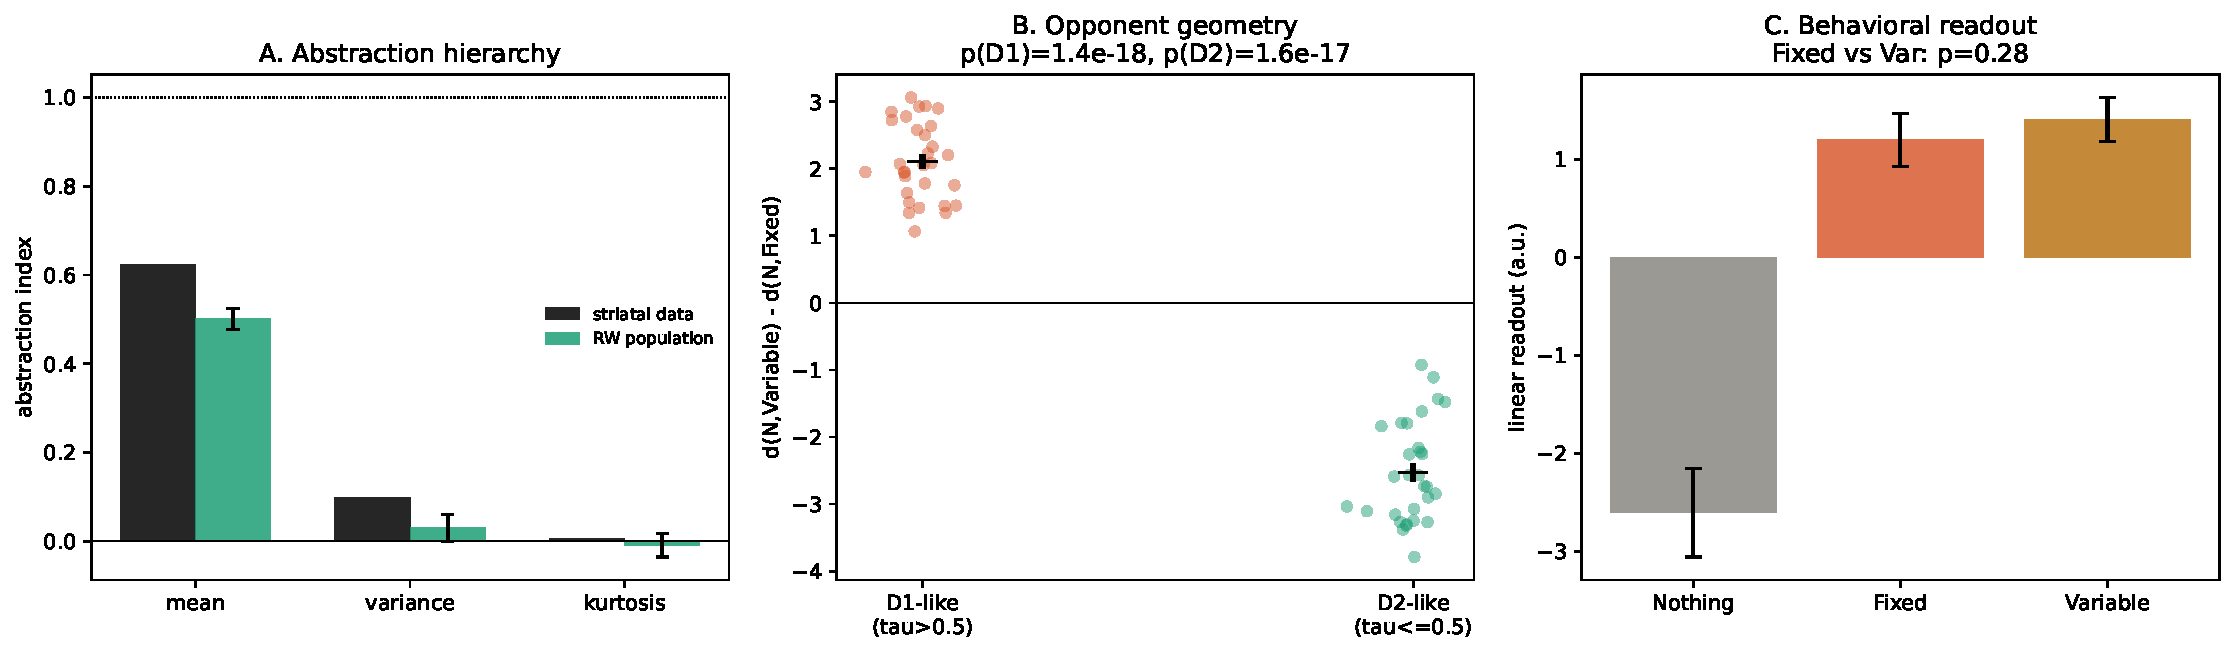
\includegraphics[width=\textwidth]{figures/01_rw_baseline.pdf}
    \caption{Baseline validation of the minimal RW population under clean (noise-free) conditions. \textbf{(A)} Abstraction index for mean, variance, and kurtosis contrasts, RW population (teal) versus real striatal recordings (black). \textbf{(B)} Opponent geometry: distance of the Nothing cue to the Variable versus Fixed cue, split by optimistic (D1-like, $\tau>0.5$) and pessimistic (D2-like, $\tau\le0.5$) subpopulations. \textbf{(C)} Linear delta-rule behavioral readout across the three cue types.}
    \label{fig:baseline}
\end{figure}

\subsection{The expectile--quantile abstraction gap grows with learning-signal noise, and only expectile sustains opponent geometry}
\label{sec:results-noise}

We next compared the expectile and quantile update rules directly, holding the population architecture fixed and varying only the update rule and the amount of noise injected into the learning signal.

Under three discrete noise conditions (clean; noisy learning signal only; noisy learning signal plus correlated observation noise calibrated from real striatal sessions), the mean-contrast AI gap between rules widened as noise was added: $+0.040$ ($p=0.078$) under clean conditions, $+0.254$ ($p<0.001$) with a noisy learning signal alone, and $+0.198$ ($p<0.001$) with both learning and observation noise (two-sample $t$-tests across $n=30$ seeds per condition; Table~\ref{tab:noise-discrete}). The variance-contrast AI showed the opposite pattern under clean conditions, with quantile numerically exceeding expectile ($-0.134$, $p<0.001$), a gap that was no longer reliable once noise was present. Kurtosis-contrast AI remained indistinguishable from chance for both rules at every noise level, as expected given its near-zero abstraction index in the empirical data.

\begin{table}[htbp]
    \centering
    \caption{Mean abstraction index (AI) by learning rule and discrete noise condition ($n=30$ seeds per cell).}
    \label{tab:noise-discrete}
    \begin{tabular}{lccc}
        \toprule
        Condition & Mean AI & Variance AI & Kurtosis AI \\
        \midrule
        Expectile, clean        & $0.796$ & $0.026$ & $-0.012$ \\
        Expectile, noisy learning & $0.816$ & $0.004$ & $-0.016$ \\
        Expectile, noisy learning + observation & $0.525$ & $0.010$ & $-0.015$ \\
        Quantile, clean         & $0.756$ & $0.160$ & $-0.018$ \\
        Quantile, noisy learning  & $0.563$ & $0.006$ & $-0.009$ \\
        Quantile, noisy learning + observation & $0.328$ & $0.007$ & $0.003$ \\
        \bottomrule
    \end{tabular}
\end{table}

A continuous sweep over learning-signal noise (SD $\in \{0, 0.5, 1.0, 1.5, 2.0, 2.5\}$, $n=15$ seeds per noise level) confirmed this as a graded, monotonic effect rather than an artifact of the discrete conditions. Expectile's mean-contrast AI was essentially flat across the noise range ($0.815 \to 0.838 \to 0.828$), while quantile's degraded steadily ($0.776 \to 0.684 \to 0.364$). The resulting expectile$-$quantile gap grew from $+0.039$ (n.s., $p=0.190$) at zero noise to $+0.464$ ($p<10^{-4}$) at the highest noise level tested, becoming significant at noise SD $\ge 0.5$ (Figure~\ref{fig:noise}A--A$'$).

The same noise sweep, applied to the D1-like/D2-like opponent-geometry metric, showed a qualitative dissociation between the two rules rather than merely a graded one. Expectile produced true opponent geometry (D1-like distance positive, D2-like distance negative) at every noise level tested, from $D1=+1.382, D2=-0.317$ at zero noise down to $D1=+0.383, D2=-0.845$ at the highest noise level. Quantile never produced opponent geometry at any noise level: its D1-like distance was negative throughout ($-2.320$ at zero noise to $-0.621$ at the highest noise level), meaning both subpopulations moved in the same direction rather than opposite directions (Figure~\ref{fig:noise}B). This indicates that the magnitude-scaled update central to the expectile rule is not merely more robust to noise in a graded sense, but is specifically what permits opponent (D1/D2-like) geometry to exist at all in this model.

\begin{figure}[htbp]
    \centering
    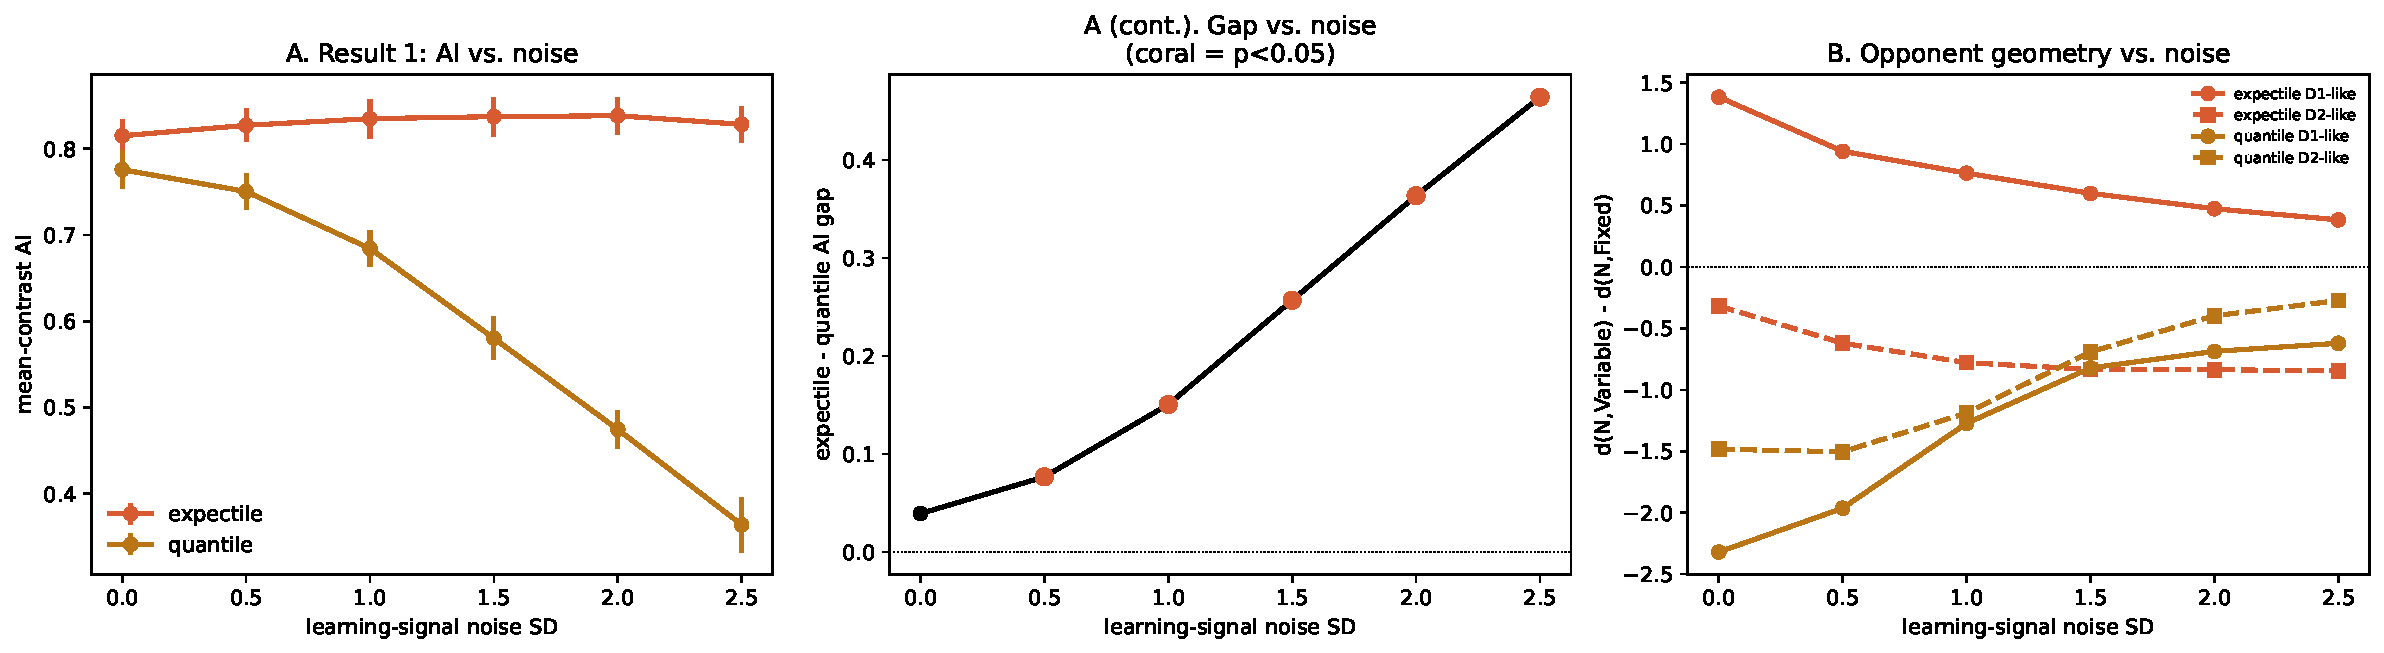
\includegraphics[width=\textwidth]{figures/02_noise_robustness.pdf}
    \caption{Noise-dependent divergence between expectile and quantile learning. \textbf{(A)} Mean-contrast abstraction index as a function of learning-signal noise, expectile versus quantile. \textbf{(A$'$)} Expectile$-$quantile AI gap versus noise; points shown in color are significant at $p<0.05$. \textbf{(B)} Opponent-geometry metric (D1-like and D2-like distances) as a function of noise, for both rules.}
    \label{fig:noise}
\end{figure}

\subsection{The expectile advantage generalizes to active decision-making across three task structures}
\label{sec:results-tasks}

To test whether the representational advantage documented above translates into behavior, we implemented a generic epsilon-greedy multi-armed bandit agent using the same tau-headed expectile or quantile value update, and evaluated it on three qualitatively different task structures, each stressing a different aspect of the update-rule distinction.

\paragraph{Non-stationary bandit.} In a four-armed bandit with abrupt shifts in which arm was best every 200 trials ($n=30$ seeds, $2000$ trials, three noise levels), expectile agents chose the optimal arm more often than quantile agents at every noise level tested (e.g.\ at noise SD $=2.0$: fraction optimal $0.59$ vs.\ $0.39$, $\Delta = +0.20$, $p<10^{-4}$), accumulated less regret ($1640.9$ vs.\ $2433.1$, $p<10^{-4}$), and recovered faster after each change point ($64.4$ vs.\ $82.6$ trials, $p<10^{-4}$; Figure~\ref{fig:task1}). These gaps were present, and if anything larger, at higher noise levels, consistent with the representational results above.

\paragraph{Gradual drift bandit.} In a four-armed bandit whose arm means drifted continuously and sinusoidally, with no discrete change points ($n=30$ seeds, $2000$ trials), the expectile agent's advantage in cumulative regret widened with noise: the gap over quantile grew from $+215.6$ (a $1.00\times$ baseline) at zero noise to $+516.1$ ($2.39\times$ the baseline gap) at the highest noise level tested. Value-tracking error (mean absolute deviation between estimated and true arm means) was consistently lower for expectile at every noise level (e.g.\ $1.209$ vs.\ $1.257$ at noise SD $=2.0$, $p<10^{-4}$; Figure~\ref{fig:task2}).

\paragraph{Risk-sensitive survival task.} In a four-armed bandit in which the highest-mean arm was also the highest-variance arm, under a depleting resource budget ($n=30$ seeds, $500$ trials), the expectile agent identified and committed to the optimal-but-risky arm substantially faster than the quantile agent at low noise (time to commit: $273.6$ vs.\ $500.0$ trials at zero noise, $p<10^{-4}$; $191.4$ vs.\ $347.2$ trials at noise SD $=1.0$, $p=0.004$). This advantage did not persist at the highest noise level tested: at noise SD $=2.0$, the gap in time-to-commit narrowed and was no longer statistically reliable ($173.7$ vs.\ $201.8$ trials, $p=0.579$), and neither the difference in fraction of optimal-arm choices ($p=0.212$) nor in survival outcomes ($p=0.322$) reached significance at that noise level (Figure~\ref{fig:task3}). This is the one task among the three in which the expectile advantage did not scale monotonically with noise, and we report it as such rather than smoothing over the discrepancy.

\begin{figure}[htbp]
    \centering
    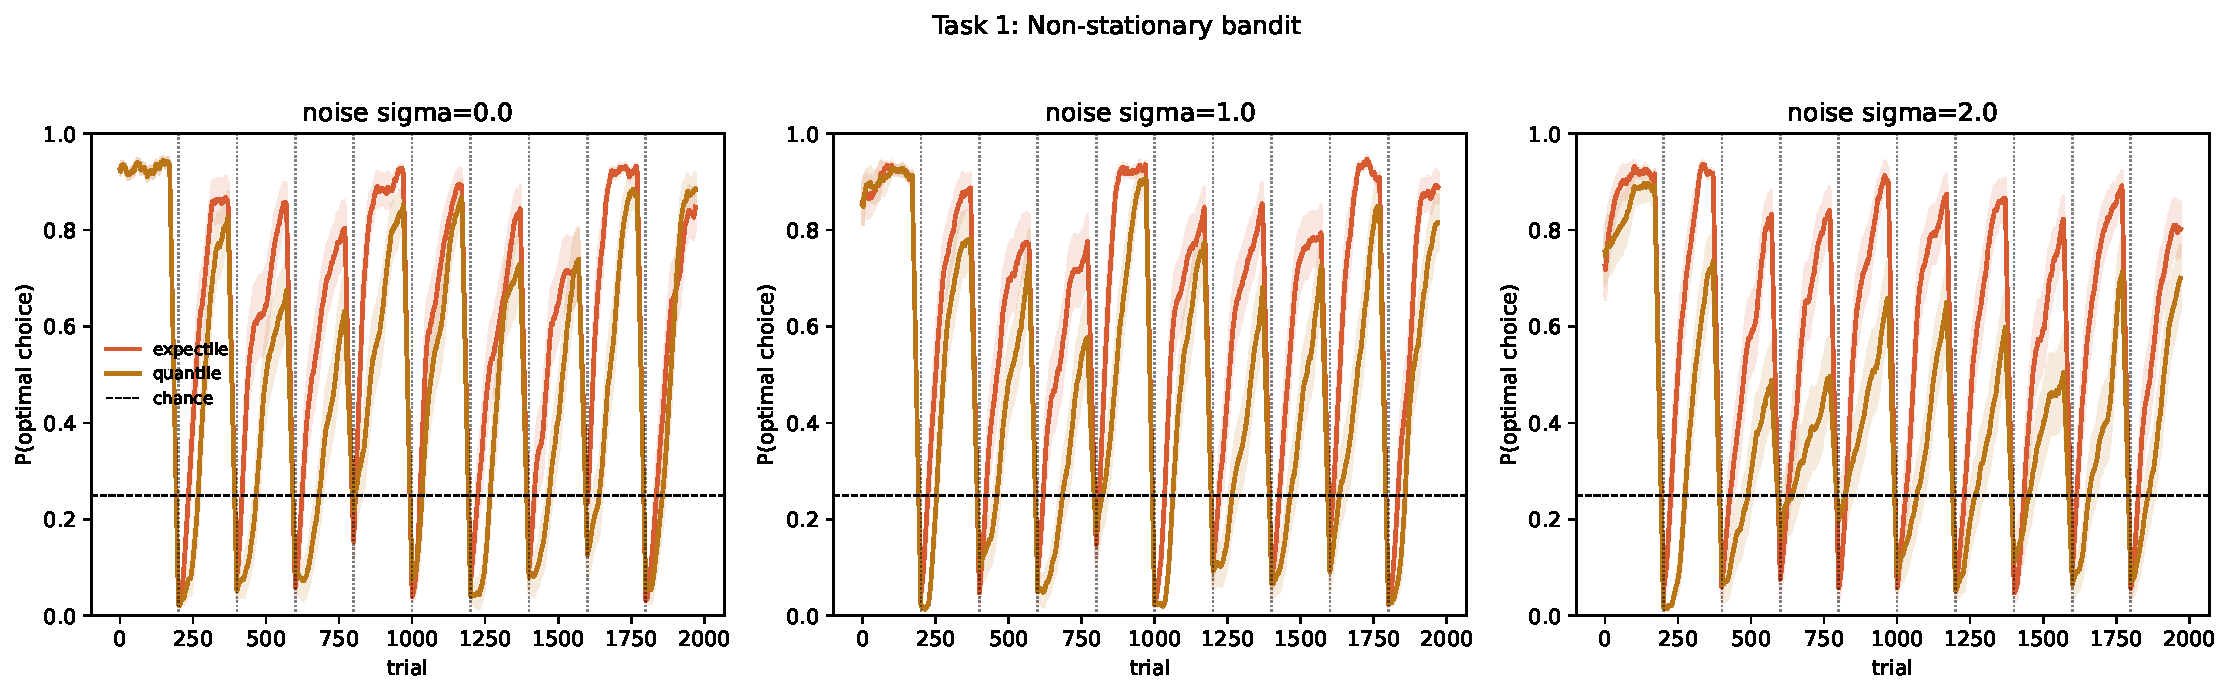
\includegraphics[width=0.85\textwidth]{figures/03_task1_nonstationary.pdf}
    \caption{Non-stationary bandit task. Fraction of optimal-arm choices over trials, expectile versus quantile, across three noise levels. Dotted vertical lines mark change points every 200 trials.}
    \label{fig:task1}
\end{figure}

\begin{figure}[htbp]
    \centering
    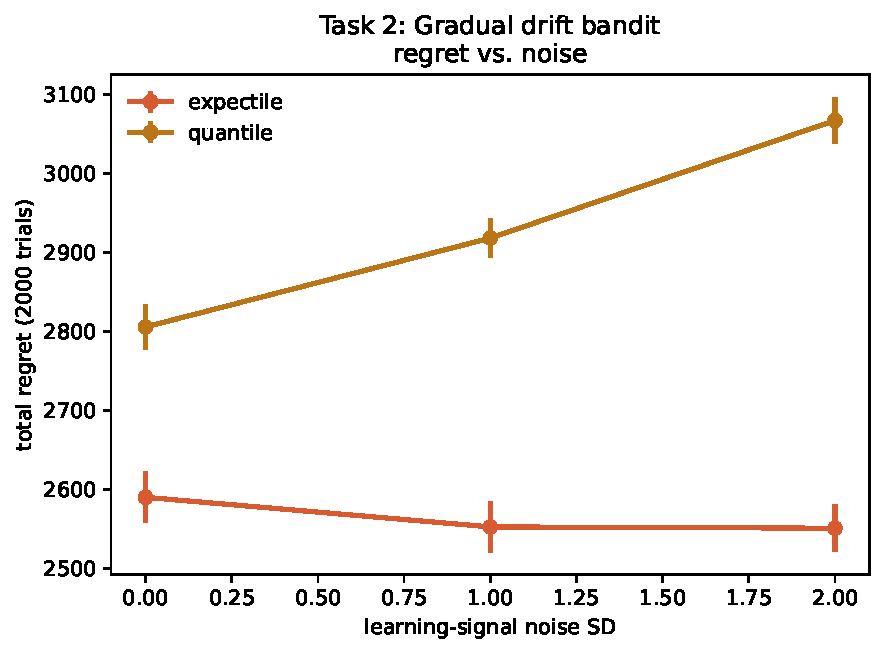
\includegraphics[width=0.6\textwidth]{figures/03_task2_drift.pdf}
    \caption{Gradual drift bandit task. Total accumulated regret over 2000 trials as a function of learning-signal noise, expectile versus quantile.}
    \label{fig:task2}
\end{figure}

\begin{figure}[htbp]
    \centering
    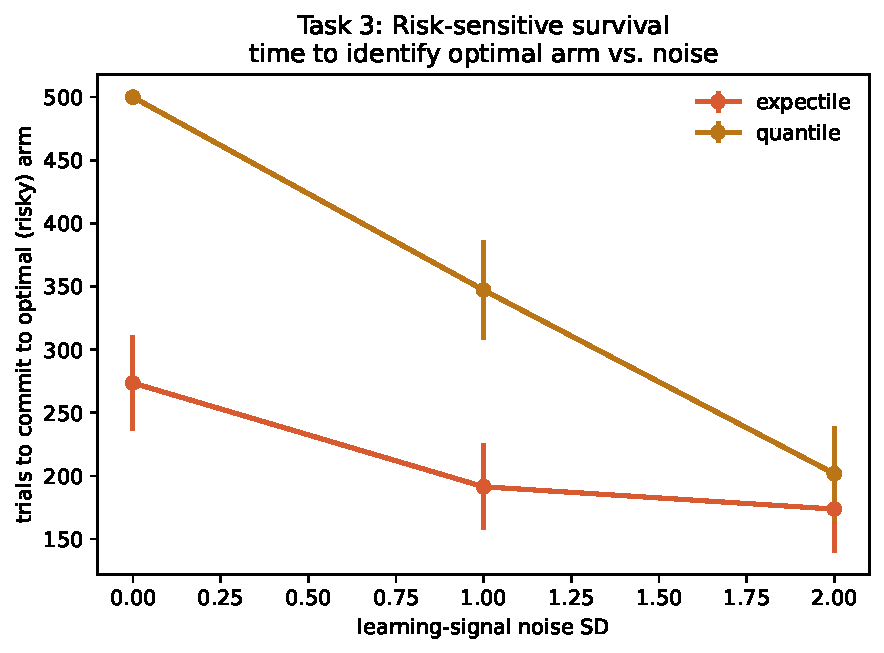
\includegraphics[width=0.6\textwidth]{figures/03_task3_risk.pdf}
    \caption{Risk-sensitive survival task. Trials required to commit to the optimal (high-mean, high-variance) arm as a function of learning-signal noise, expectile versus quantile.}
    \label{fig:task3}
\end{figure}

\section{Methods}
\label{sec:methods}

\subsection{Empirical calibration data}
\label{sec:methods-empirical}

All simulations below are calibrated against, but do not directly re-analyze, the striatal Neuropixels recordings of \citet{lowet2025}, obtained from the associated Dryad repository. Two of the three published datasets were used: \emph{SameRewDist} (13{,}997 neurons, 71 sessions, 12 mice; six odor cues instantiating Nothing/Fixed/Variable reward distributions) and \emph{SameRewVar} (6{,}816 neurons, 32 sessions, 5 mice; six odor cues instantiating Uniform/Bimodal reward distributions matched on mean and variance). The third published dataset (two-photon D1/D2 imaging) was not used, since the D1/D2-like opponent-geometry result in this work is derived entirely from the model (Section~\ref{sec:results-baseline}) rather than from the imaging data.

From these recordings we extracted only the small set of scalar and matrix quantities needed to calibrate the simulations, rather than re-analyzing the recordings themselves: (i) a reference abstraction-index hierarchy for the mean, variance, and kurtosis contrasts, computed per session with the same cross-condition-generalization decoding procedure described in Section~\ref{sec:methods-decoding} and averaged across sessions ($n=64$ sessions for mean and variance, $n=31$ for kurtosis); (ii) an empirical trial-to-trial observation-noise correlation matrix, estimated from residual (mean-subtracted) activity of 20 randomly sampled medium spiny neurons (MSNs) per session and trial type, pooled across 384 session$\times$trial-type pairs (mean off-diagonal correlation $= 0.037$), tiled to the simulated population size, regularized to be positive definite, and Cholesky-factorized; and (iii) the median number of valid trials per condition per session (35) and the median number of MSNs per session (88), used to set the trial count and population size in the simulations below.

\subsection{Minimal Rescorla--Wagner population}
\label{sec:methods-rw-population}

The core model is a population of $N=50$ independent scalar value-learning units, indexed by cue $c \in \{1,\dots,6\}$ (two cues per reward distribution, as in the real task) and unit $i \in \{1,\dots,N\}$. Each unit $i$ has an asymmetric learning-rate pair $(\alpha_i^+, \alpha_i^-)$, parameterized by an effective expectile level $\tau_i \sim \mathrm{Uniform}(0.05, 0.95)$ via $\alpha_i^+ = 2 \rho \tau_i$, $\alpha_i^- = 2\rho(1-\tau_i)$, with base rate $\rho = 0.05$. On each trial, a cue $c$ is presented, a reward $r$ is drawn from that cue's distribution, and the prediction error $\delta_i = r - V_{c,i}$ updates the unit's value estimate under one of two rules:
\begin{align}
    \text{expectile:} \quad & V_{c,i} \leftarrow V_{c,i} + \alpha_i^{\mathrm{sgn}(\delta_i)} \, \delta_i, \\
    \text{quantile:} \quad & V_{c,i} \leftarrow V_{c,i} + \alpha_i^{\mathrm{sgn}(\delta_i)} \, \mathrm{sgn}(\delta_i),
\end{align}
where $\alpha_i^{\mathrm{sgn}(\delta_i)}$ denotes $\alpha_i^+$ if $\delta_i > 0$ and $\alpha_i^-$ otherwise. The expectile rule scales the update by the magnitude of the prediction error, corresponding to an asymmetric squared loss \citep{newey1987,rowland2019}; the quantile rule takes a fixed-size step in the direction of the error only, corresponding to an asymmetric absolute-value (pinball) loss. Units with $\tau_i > 0.5$ are termed ``D1-like'' (optimistic, upweighting positive errors); units with $\tau_i \le 0.5$ are termed ``D2-like'' (pessimistic).

For analyses requiring a realistic trial-count regime (Sections~\ref{sec:results-baseline}--\ref{sec:results-noise}), each cue was presented 35 times per simulated ``session'' in randomly interleaved order (matching the empirical median trial count, Section~\ref{sec:methods-empirical}), and the population's value estimate was probed (with added observation noise) on the last 17 presentations of each cue, yielding one simulated pseudo-trial per probe. For analyses requiring converged values only (opponent-geometry and behavioral-readout analyses in Section~\ref{sec:results-baseline}), the population was instead trained for 30{,}000 trials with no probing or observation noise.

Two sources of noise were applied, independently or jointly: (i) \emph{learning-signal noise}, Gaussian noise with standard deviation $\sigma_{\mathrm{learn}}$ added to the reward $r$ before computing $\delta_i$ (but not to the reward used elsewhere), modeling a corrupted teaching/prediction-error signal; and (ii) \emph{observation noise}, added to the probed value estimates only, either independently ($\mathcal{N}(0, \sigma_{\mathrm{obs}}^2)$ per unit, $\sigma_{\mathrm{obs}} = 5$) or with the empirically calibrated correlation structure (Section~\ref{sec:methods-empirical}) via its Cholesky factor $L$, as $L z$ with $z \sim \mathcal{N}(0, I)$.

\subsection{Decoding, abstraction index, and opponent geometry}
\label{sec:methods-decoding}

Population geometry was quantified with a cross-condition-generalization procedure (CCGP), matching the decoding approach used on the real recordings. For a contrast with two cues signaling each of two conditions (e.g.\ Nothing$_1$/Nothing$_2$ versus Fixed$_1$/Fixed$_2$), a linear support vector classifier (linear kernel, $C=5\times10^{-3}$, balanced class weighting) was trained on one cue pairing and tested on the other, and vice versa, with the resulting balanced accuracy averaged across both directions and both possible pairings (\emph{cross}-identity accuracy). A matched within-identity accuracy (\emph{within}) was obtained by 5-fold cross-validation on a single cue pairing. Each condition was bootstrap-resampled to 200 pseudo-trials before decoding. The abstraction index was defined as
\begin{equation}
    \mathrm{AI} = \frac{\mathrm{cross} - 0.5}{\mathrm{within} - 0.5},
\end{equation}
with $\mathrm{AI} \approx 1$ indicating fully abstract (odor-independent) coding and $\mathrm{AI} \approx 0$ indicating decodable but odor-specific coding. The same procedure was applied to three contrasts in each dataset: mean (Nothing vs.\ Fixed), variance (Fixed vs.\ Variable), and kurtosis (Uniform vs.\ Bimodal, using the \emph{SameRewVar}-analog reward distributions in simulation).

Opponent geometry was quantified as $d(N,\mathrm{Var}) - d(N,\mathrm{Fix})$, the difference in Euclidean distance (in $z$-scored value space, normalized within each subpopulation) between the Nothing cue and the Variable versus Fixed cues, computed separately for D1-like ($\tau>0.5$) and D2-like ($\tau\le0.5$) subpopulations.

\subsection{Behavioral readout}
\label{sec:methods-readout}

A scalar behavioral readout was obtained by training a linear delta-rule weight vector $w$ on top of the ($z$-scored) converged population values, $w \leftarrow w + \eta (r - w^\top V_c) V_c$, for $10{,}000$ trials with learning rate $\eta=0.01$, and evaluating the resulting readout $V_c^\top w$ for each cue.

\subsection{Bandit agent and task designs}
\label{sec:methods-tasks}

For the active-decision-making experiments (Section~\ref{sec:results-tasks}), we used a generic $\varepsilon$-greedy ($\varepsilon=0.1$) multi-armed bandit agent with the same expectile/quantile tau-headed value update described in Section~\ref{sec:methods-rw-population} ($10$ $\tau$-heads per arm, linearly spaced on $[0.05, 0.95]$), choosing on each trial the arm with the highest mean estimate across $\tau$-heads (or a random arm with probability $\varepsilon$).

\paragraph{Non-stationary bandit.} Four arms with fixed variances ($0, 2, 4, 6$) and means that shifted abruptly every 200 trials, with the identity of the best arm (mean $+2$ above the other three) rotating deterministically; $2000$ trials, learning rate $0.15$, $n=30$ seeds per condition, learning-signal noise SD $\in \{0, 1, 2\}$.

\paragraph{Gradual drift bandit.} Four arms with fixed variances ($0.5, 1, 2, 3$) whose means drifted sinusoidally and continuously ($\mathrm{mean}_a(t) = 4 + 2\sin(2\pi t / 400 + a\pi/2)$ for arm $a$), with no discrete change points; $2000$ trials, learning rate $0.05$, $n=30$ seeds per condition, same noise levels as above.

\paragraph{Risk-sensitive survival task.} Four arms: a safe suboptimal arm (mean $4.2$, variance $0$), an optimal but high-variance arm (mean $5.0$, variance $9$), a below-cost arm (mean $3.8$, variance $0$), and a moderate-variance distractor (mean $4.0$, variance $4$), under a depleting resource budget (initial budget $30$, cost $4$/trial, with reward added each trial); the agent's estimated time to commit to the optimal arm was defined as the first trial after which that arm was chosen for 10 consecutive trials; $500$ trials, learning rate $0.05$, $n=30$ seeds per condition, same noise levels as above. This design is motivated by evidence that ventral striatal circuits, and D2-expressing MSNs in particular, are causally implicated in risky decision-making \citep{costa2016,zalocusky2016}, and by risk-sensitive reinforcement-learning formulations that explicitly separate value from risk \citep{shen2014,tamar2015}.

\subsection{Statistics}
\label{sec:methods-stats}

All comparisons between expectile and quantile rules were two-sample $t$-tests across independent random seeds (number of seeds given per analysis above); comparisons of a single quantity against a null value of zero (e.g.\ opponent-geometry distances) were one-sample $t$-tests. No corrections for multiple comparisons were applied, given the exploratory and descriptive (rather than confirmatory) role of these analyses relative to the primary noise-scaling result in Section~\ref{sec:results-noise}.

\section{Discussion}
\label{sec:discussion}

We asked whether there is a reason, beyond shared asymptotic validity, for a biological learning circuit to implement expectile rather than quantile distributional RL. Across a minimal population model, a direct sweep over learning-signal noise, and three qualitatively different active decision tasks, the answer was consistently yes, but in a specific and graded form rather than a blanket one: expectile's advantage over quantile in preserving mean-value coding was small and often unreliable under clean conditions, widened monotonically as learning-signal noise increased (Section~\ref{sec:results-noise}), and generalized to faster tracking, lower regret, and (mostly) faster identification of valuable-but-risky options in active tasks (Section~\ref{sec:results-tasks}). A second, more categorical result accompanied this graded one: D1-like/D2-like opponent geometry was present under the expectile rule at every noise level tested and absent under the quantile rule at every noise level tested (Section~\ref{sec:results-noise}). The same magnitude-scaled update that buys robustness to noise is, in this model, also what makes opponent coding possible at all.

\paragraph{A general, not neuroscience-specific, mechanism.} The expectile and quantile update rules used here differ in exactly one respect: expectile scales its update by the magnitude of the prediction error, while quantile reduces the error to its sign and takes a fixed-size step. This is the same distinction that separates ordinary stochastic gradient descent from sign-based optimizers such as signSGD in machine learning \citep{bernstein2018}. That literature has already established, independently of any biological motivation, that discarding gradient magnitude trades away exactly the kind of noise robustness we observe here: sign-based updates are attractive for their communication and memory efficiency, but they systematically underperform magnitude-aware updates once the gradient (or, in our setting, the reward-prediction-error) signal itself is corrupted by noise. Our result can therefore be read as a specific instance of a more general principle rather than a fact about dopamine or the striatum per se: whenever a system must learn from a noisy scalar teaching signal under a fixed step budget, discarding the magnitude of that signal is costly, and the cost grows with the noise.

\paragraph{Reconciling with the statistics literature on expectile and quantile regression.} A body of work on \emph{static} expectile and quantile regression reaches an apparently opposite conclusion: quantile regression's $\ell_1$-type loss is generally considered more robust to outliers and heavy-tailed contamination than expectile regression's $\ell_2$-type loss \citep{newey1987,waltrup2015}. We do not think this contradicts our finding, because the two literatures ask different questions about different objects. The classical result concerns robustness of a \emph{one-shot fit} to heavy tails or contamination in the \emph{target distribution itself} --- a squared loss is sensitive to occasional extreme observations because large errors are up-weighted quadratically. Our manipulation instead corrupts the \emph{teaching signal} used in a \emph{sequential} update around an otherwise well-behaved (Gaussian or two-point) target, and does so at every step rather than as rare contamination. In that setting, a fixed-size step cannot distinguish a trustworthy error from an untrustworthy one and is therefore driven by noise on every trial, whereas an error-scaled step naturally shrinks when the current estimate is already close to (a noisy realization of) the target. The two results are complementary rather than contradictory: expectiles are the worse choice for fitting a single heavy-tailed batch of data, but may be the better choice for online learning from a noisy but otherwise well-behaved stream --- precisely the regime a biological RPE signal plausibly occupies.

\paragraph{Relation to existing normative accounts of D1/D2 opponency.} \citet{jaskirfrank2023} offer a normative account of dynamic D1/D2 modulation grounded in the statistics of the \emph{environment}: opponent, richness-dependent gain on the Go/No-Go pathways corrects a specific pathology of sparse-reward environments, in which sampling noise alone can make an optimal option's estimated value drop below a suboptimal one's. Our account is grounded instead in noise internal to the \emph{learning signal}, and in a task structure (matched-mean, differing-variance cues) in which the environment's reward rate is not the relevant statistic. These are not competing explanations for the same phenomenon; they are two different selective pressures that could both favor the same architecture, operating at different timescales (online gain modulation in their model; a fixed asymmetry in ours) and under different environmental regimes (reward sparsity there; teaching-signal noise here). A natural extension would combine both regimes in one model to ask whether they trade off, reinforce each other, or dominate in different parts of parameter space --- something the present work, which holds environmental reward rate fixed, cannot address.

\paragraph{The risk-sensitive task did not confirm a monotonic advantage.} Two of our three active tasks showed the same noise-scaling pattern found in the representational analyses: the expectile agent's advantage over quantile grew, or at minimum did not shrink, as noise increased. The risk-sensitive survival task was the exception: the expectile agent's advantage in identifying the optimal-but-risky arm was largest at zero noise and was no longer statistically reliable at the highest noise level tested (Section~\ref{sec:results-tasks}). We see at least two non-exclusive explanations. First, this task couples value learning to a resource budget with an absorbing failure state (running out of budget), which introduces task dynamics --- variance in survival itself, floor effects on trials remaining once budget is low --- that are absent from the other two tasks and could mask a representational advantage that is nonetheless still present. Second, it is possible that the noise-robustness advantage genuinely does not extend to identifying a specific high-variance option under time pressure, as opposed to tracking a scalar mean, and that this constitutes a real boundary condition on the claim rather than a measurement artifact. We do not adjudicate between these here and flag it as the clearest open question raised by this work, rather than omit or reframe the result to fit the pattern found elsewhere.

\paragraph{Limitations.} The model is a population of independent scalar Rescorla--Wagner units, not a spiking or biophysically detailed circuit, and the D1-like/D2-like split is inferred post hoc from the sign of each unit's effective expectile level rather than built in as a separate anatomical constraint; this mirrors the logic of REDRL \citep{lowet2025} but runs in the opposite inferential direction (asymmetry $\to$ opponency, rather than opponency $\to$ asymmetry), and we do not independently verify that D1/D2 MSNs recorded under experimentally elevated noise actually show the predicted geometry. The three active tasks are synthetic multi-armed bandits chosen to isolate specific computational demands (abrupt change, continuous drift, risk under budget pressure) rather than fit to any specific animal behavioral dataset. Population size, learning rate, and $\tau$-distribution shape were calibrated once against real striatal recordings (Section~\ref{sec:methods-empirical}) rather than swept as free parameters throughout, so we cannot yet rule out that some noise-robustness gaps are sensitive to this specific calibration.

\paragraph{Reframing the empirical claim.} Taken together, these results reframe the relationship between \citet{lowet2025}'s empirical finding and its algorithmic explanation. Rather than treating expectile-based REDRL as simply the model that best \emph{fits} the observed striatal geometry, our results suggest a reason the striatum would be \emph{favored} to land on something like it: under learning-signal noise of the kind directly measured in reward-guided learning \citep{findling2019}, an expectile-like update preserves both value estimation and the specific opponent geometry that a two-cell-type circuit can express, while a quantile-like update does neither reliably. This is a causal, adaptive argument layered on top of a descriptive match, and it generates a directly testable prediction for future recordings: if the noise-robustness account is correct, sessions or animals with noisier reward-prediction-error signals should show more pronounced D1/D2 asymmetry, not less, whereas an account based purely on environmental reward statistics predicts no such relationship.

\bibliographystyle{apalike}
\bibliography{references}

\end{document}
